\documentclass[handout]{beamer}
%\documentclass[xcolor=pst]{beamer}
%\usepackage[spanish]{babel}
\usepackage[utf8]{inputenc}

\usepackage{amssymb,amsmath}
\usepackage{bbm}
\usepackage{graphicx}
%\usepackage[pdf]{pstricks}
\usepackage{colortbl}
\definecolor{fucsia}{rgb}{1,0,1}
%\usepackage[Q=yes]{examplep}

\newcounter{savedenum}
\newcommand*{\saveenum}{\setcounter{savedenum}{\theenumi}}
\newcommand*{\resume}{\setcounter{enumi}{\thesavedenum}}

%\usepackage{default}
\usetheme{Madrid}

%\setbeamertemplate{caption}[numbered]


\title[L-Shape Selection]{A heuristic algorithm to select genes potentially regulated by methylation}
\author[Alex S\'anchez]{Alex S\'anchez, Berta Mir\'o, Francesc Carmona, \\
	Sarah Bazzoco and Diego Arango del Corro}
\date[]{July 09, 2018}

\begin{document}
\begin{frame}
	
\begin{scriptsize}
\begin{center}
  \emph{ XXIX International Biometric Conference (IBC2018)}
\end{center}
\end{scriptsize}

\titlepage

\begin{columns}
   \column{0.7\textwidth}
   \scriptsize
   Genetics, Microbiology and Statistics Department \\ 
   \textbf{Facultad de Biología, Universitat de Barcelona}\\
   Statistics and Bioinformatics Unit (UEB)\\
   Department Molecular Oncology-CIBBIM \\ 
   \textbf{Vall Hebron Institut de Recerca}

  \hfill\column{0.3\textwidth}
  
\includegraphics[height=1cm]{images/alllogos.png}
% 
\includegraphics[height=0.5cm]{images/VHIR_fonstransp.png}
\end{columns}

\end{frame}


\begin{frame}
\frametitle{Table of Contents}
\tableofcontents
\end{frame}

\section{Introduction / Motivation}

\subsection{Genome-wide analysis of colorectal cancer}

\begin{frame}
	\frametitle{Genome-wide analysis of colorectal cancer}
	  \begin{itemize}
	  	\item This work started as collaboration with a Molecular Oncology group working on Colorectal Cancer (CRC).
	  	\item CRC is a serious public health problem (2.M diagnosed/year) but the number of therapies available is smaller than in other cancer types.
	  	\item Researcher's interest: identification of biomarkers for chemotherapy sensitivity.
	  	%\item The study analyzed a panel of 30--45 cell lines derived from colorectal tumors characterized by increasing sensitivity to several chemotherapy drugs (Irinotecan, Cetuximab, Oxaliplatin).
	  	\item The researchers' approach was to look for \textit{genes regulated by methylation} which could be considered possible therapeutic targets.
	  	\end{itemize}
\end{frame}

\begin{frame}
	\frametitle{Methylation}
	\begin{itemize}
		\item Methylation of CpG dinucleotides in the promoter of genes
		involved in the oncogenic process has been shown to be a key process
		contributing to tumor initiation and/or progression.
		\item Essentially (and especially in cancer) methylation acts by inhibiting gene expression that
		is,\emph{ the more methylated is a gene the more repressed is its expression}
		\begin{center}
			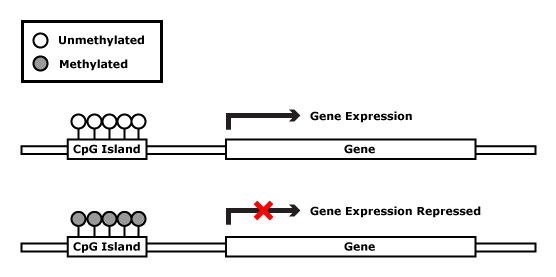
\includegraphics[width=0.7\textwidth]{./images/methylationAction1.png}
		\end{center}
	\end{itemize}
\end{frame}

\begin{frame}{Patterns of (negative) association}
	\begin{itemize}
		\item Considering the relation between methylation and expression in cancer (the higher methylation the lower the expression...)
		\item leads to expecting that scatterplots depicting the relation between methylation and expression show a negative correlation.
		\item This is usually the case and, indeed, \textit{genes known to be regulated by methylation often show \textbf{an L-shape pattern} in these plots}.
	\end{itemize}
	\begin{center}
		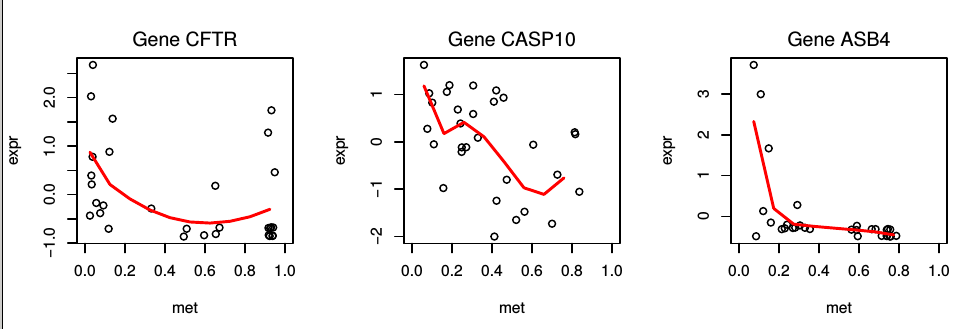
\includegraphics[width=0.7\textwidth]{./images/Lshapes1.png}
	\end{center}
\end{frame}

\begin{frame}{Selecting genes by mining scatterplots}
	\begin{itemize}
		\item Assuming the relation described above is true...
		\item Finding genes regulated by methylation is equivalent to finding genes whose methylation--expression scatterplot has an L--shape.
		\item There is a scatterplot \emph{per} gene and thousands of genes:\\ {\emph{Automatic methods for selecting interesting genes through their scatterplots are required}}.
		\item There exist methods  that add on the correlation coefficient but they are not very successful.
	\end{itemize}
\end{frame}


\subsection{Objectives}

\begin{frame}
	\frametitle{Objectives}
	
The main objectives of this work are:
\begin{enumerate}
	
	\item To introduce a new method to select genes showing an L-shape
	\item To compare it with previously available methods, 
	\item To apply the selected methods on a specific CRC dataset and validate the findings based on their biological relevance.
	
\end{enumerate}

\end{frame}

\section{Methods for selecting L-shaped patterns}

\begin{frame}
\frametitle{Previously applied methods}

%	\begin{itemize}
%		\item Naive method: Call regulated by methylation genes depictinhg negative correlation between expression and methylation
%		\item Study variation of conditional mutual information along different methylation values.\cite{Liu:2012}.
%		\item Use regression splines to fit a curve to the scatterplot and use clustering to group patterns. \cite{Sanchez:2017}.
%		\item Analyze scatterplots characteristics with Tukey's Scagnostics method \cite{Wilkinson:2017}
%	\end{itemize}

\begin{center}
	\begin{figure}[h]          
		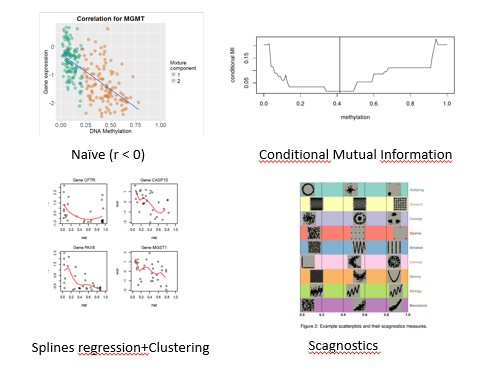
\includegraphics[width=0.9\textwidth]{images/otherMethods.png}
	\end{figure}
\end{center}


\end{frame}

\subsection{A new algorithm}

\begin{frame}
	\frametitle{What is an L-shape, whatsoever}
\begin{columns}%
	\begin{column}[t]{0.5\textwidth}%
		\bigskip
		\begin{itemize}
			\item Go back to an intuïtive idea
		%	\item \emph{``L-shaped'' genes should show an L shape in the scatterplot}; 
		%		\begin{itemize}
				
					\item The more the values in the scatterplot move away from the axes the least L-shaped the gene is.
					
					\bigskip
					\bigskip
					\bigskip
					\item The more the values cluster near the  vertical and horizontal axes, the more L-shaped can be considered the scatterplot.
		%		\end{itemize}
		\end{itemize}
		
	\end{column}
	\begin{column}[t]{0.5\textwidth}%
		\begin{center}
			\begin{figure}[h]          
				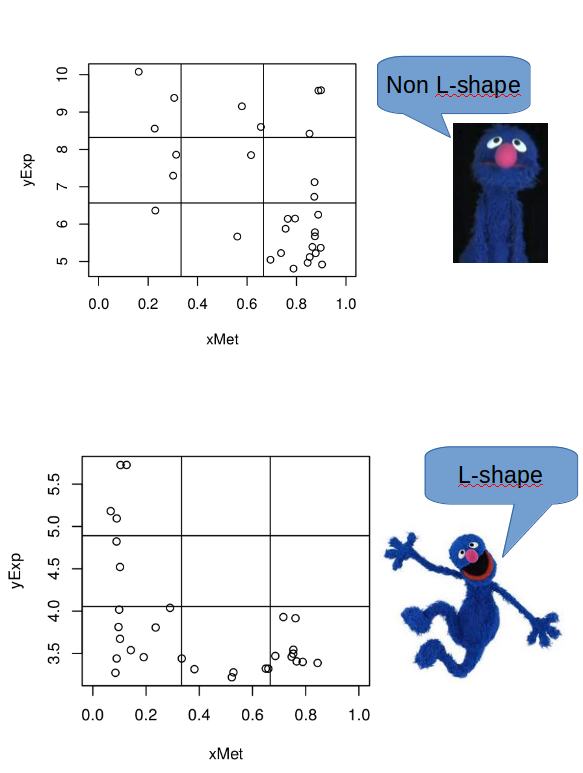
\includegraphics[height=0.8\textheight]{images/LshapeNonLshape.png}
			\end{figure}
		\end{center}
	\end{column}
\end{columns}	
\end{frame}

\begin{frame}
	\frametitle{A penalization system}
	\begin{enumerate}
		\item Overimpose a $3\times 3$ grid on the scatterplot.
		\item Classify the scatterplot as \textbf{``L'' or ``non-L''} based on a small set of conditions:
		\begin{enumerate}
			\item There must be a \emph{minimum} number of points in the left and lower cells of the grid.
			\item There must be a \emph{maximum} number of points in the upper region (points there mean hypermethylation and hyperexpression, the opposite of what we are looking for).
		%	\item We will usually \emph{not require to have a minimum of points in cell (3,1)} unless we are really willing to have an L-shape (in our setting we will also be happy tho recover diagonals, which also reflect a negative correlation!).
		\end{enumerate}
	\end{enumerate}
{
\begin{equation*}
\mathbbm{1}_L(X) = \bigwedge_{i,j} X \circ C \circ \left( mMP \times \sum_{i,j}x_{ij}\right),
\end{equation*}
}

\end{frame}

\begin{frame}
	\frametitle{A scoring system}
		\begin{enumerate}
			\item Score points on each subgrid in such a way that
			\begin{enumerate}
				\item Points in permitted regions (left-outer margin, i.e. cells: (1,1), (2,2), (3,1), (3,2), (3,3)) score positively if the scatterplot has been classified as L or zero if it has been classified as non-L.
				\item Points in non-desired regions (outer band. i.e. cells (1,2), (1,3), (2,3)) score negatively in all cases.
				\item Some regions may be declared neutral and not-score, such as cell (2,2).
			\end{enumerate}
			{
			\begin{equation*}
			S(X) = W_L \circ X \times \mathbbm{1}_L(X) + W_{L^C} \circ X \times \mathbbm{1}_{L^c}(X),
			\end{equation*}
		    }
			\item Use cross-validation to tune scoring parameters (\emph{if a set of positive and negative L-shaped genes is available}).
		\end{enumerate}
	

\end{frame}



\begin{frame}
	\frametitle{An example}

\begin{columns}%
	\begin{column}[t]{0.4\textwidth}%	

\begin{enumerate}

\item Min-Max Counts
$$
mMP =\left(\begin{smallmatrix}
	10 & 20 & 0\\ 
	5 & 30 & 20\\ 
	0 & 5 & 5
\end{smallmatrix}\right)
$$

\item Matrix of weights for TRUE L scatterplots
$$
W_{TRUE-L} =\left(\begin{smallmatrix}
2 & -2 & -25\\ 
1 & 0 & -2\\ 
1 & 1 & 2
\end{smallmatrix}\right)
$$

\item Matrix of weights for FALSE L scatterplots
$$
W_{FALSE-L} =\left(\begin{smallmatrix}
0 & -2 & -25\\ 
0 & 0 & -2\\ 
0 & 0 & 0
\end{smallmatrix}\right)
$$

\end{enumerate}

	\end{column}
	\begin{column}[t]{0.6\textwidth}%
		\bigskip
		\begin{center}
			\begin{figure}[h]          
				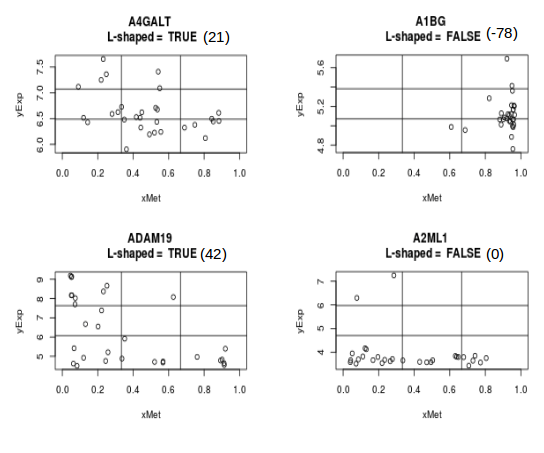
\includegraphics[width=\textwidth]{images/LshapeAndNonLshapeScored}
			\end{figure}
		\end{center}
	\end{column}
\end{columns}	
	
\end{frame}

\section{Results and Applications}

\begin{frame}[allowframebreaks]
	\frametitle{Data for the comparisons}
	\begin{itemize}
		\item The methods have been tested using three real and one simulated dataset.
		\item Distinct datasets were generated by similar but not identical technologies.
		\item Genes non common to the three datasets were removed from the analysis
	\end{itemize}
\begin{table}[]
	\begin{tabular}{|l|l|c|c|l|l|}
		\hline
		\textit{Name} & \textit{Source} & \multicolumn{1}{l|}{\textit{Genes}} & \multicolumn{1}{l|}{\textit{Samples}} & \textit{Arrays}   & \textit{Methylation} \\ \hline
		\textbf{TCGA} & Nature 2012     & 11788                                & 223      &  Agilent                  &  Illumina 27K                    \\ \hline
		\textbf{GEO}  & GSE25070        & 11191                &  25            & Agilent & Illumina 27K        \\ \hline
		\textbf{DA}   & Researcher's    & 11359                               & 30                                    & Affymetrix & Illumina 27K       \\ \hline
	\end{tabular}
\end{table}	

\framebreak

\begin{center}
	\begin{figure}[h]          
		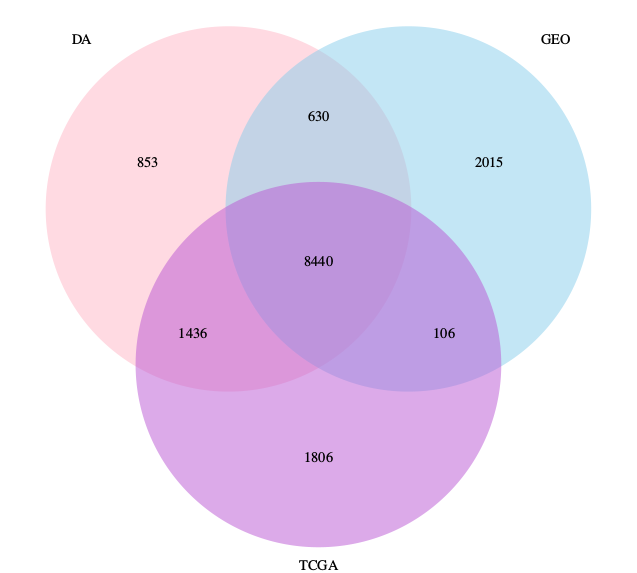
\includegraphics[height=0.8\textheight]{images/genesInCommonBetweenDatasets.png}
	\end{figure}
\end{center}

\end{frame}

\begin{frame}
\frametitle{Results: Pathway Analysis of selected genes}
Two types of pathway analysis are undergoing
\begin{enumerate}
	\item \textit{Gene Enrichment Analysis} on each of the three gene lists analyzed. \newline
	This analysis yields a set of functional categories
	\begin{itemize}
		\item How similar are the gene sets obtained from the analysis?
		\item \textit{Which of these sets suggest there is regulation by methylation?}
	\end{itemize}
	\item \textit{Pathway Equivalence Analysis} (\texttt{goProfiles}) of the three gene lists complemented with a three more random lists of same sizes. 
	\begin{itemize}
	\item Are the lists equivalent in their GO categories representation?
	\item Are they more similar to each other than to random selected lists from the corresponding sets?
	\end{itemize}
\end{enumerate}
\end{frame}

\begin{frame}
	\frametitle{Results: Comparison between datasets}
\begin{center}
	\begin{figure}[h]          
		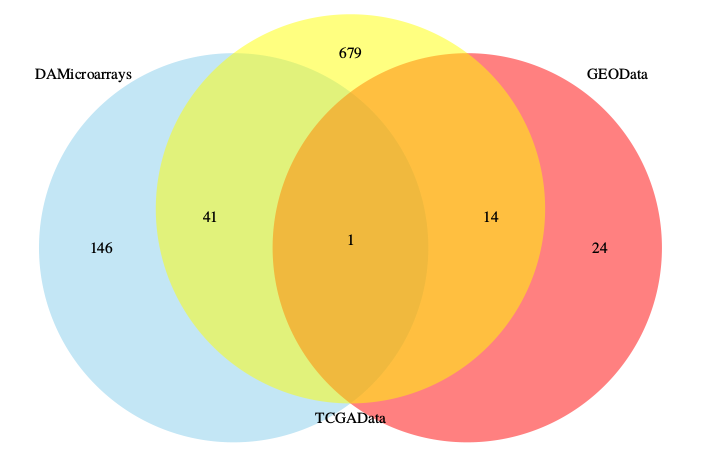
\includegraphics[height=0.8\textheight]{images/genesInCommonBetweenHEURISTICselections.png}
	\end{figure}
\end{center}
\end{frame}


\begin{frame}
	\frametitle{Results: Comparison between the methods}
\begin{center}
	\begin{figure}[h]          
		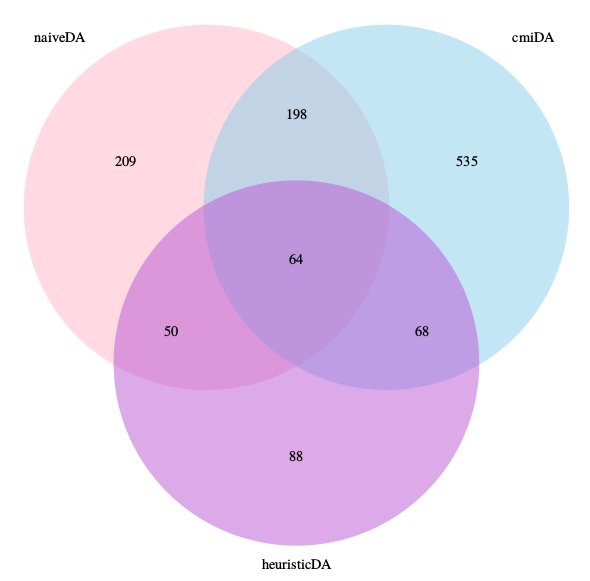
\includegraphics[height=0.8\textheight]{images/genesInCommonBetweenMethodsInDA.png}
	\end{figure}
\end{center}
\end{frame}

\begin{frame}
\frametitle{Results: Pathway Analysis}
\begin{center}
	\begin{figure}[h]          
		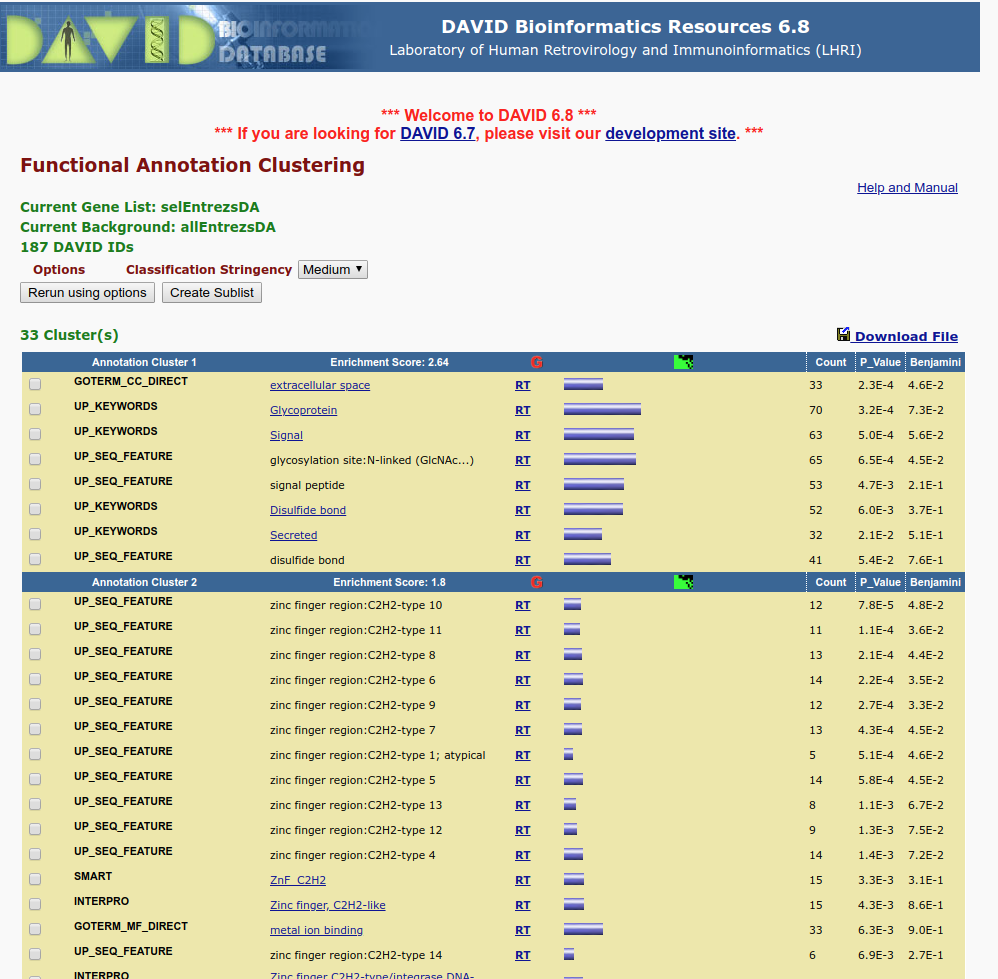
\includegraphics[height=0.8\textheight]{images/DAVID-Analysis-DAList.png}
	\end{figure}
\end{center}
\end{frame}



\frame[allowframebreaks]{\frametitle{Software}
	\begin{center}
		\begin{figure}[h]          
			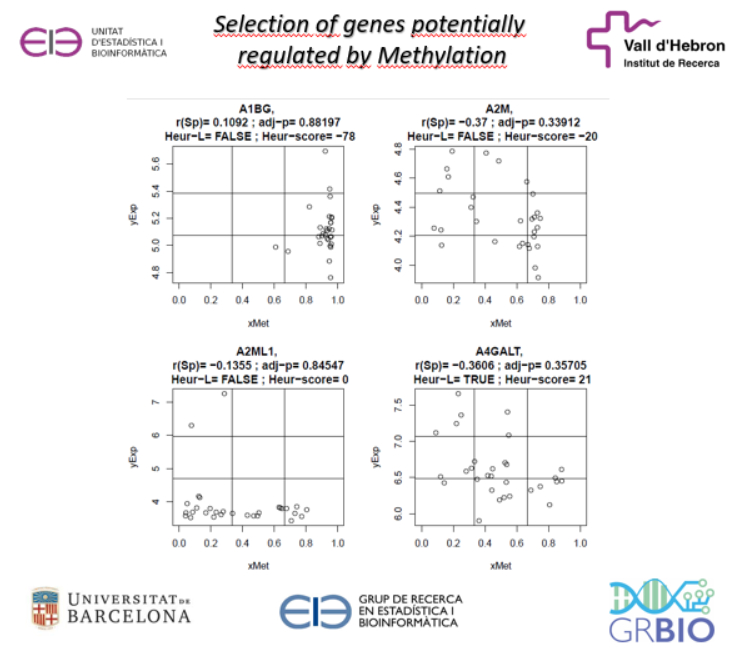
\includegraphics[height=0.8\textheight]{images/shinyApp1.png}
		\end{figure}
	\end{center}

	\begin{center}
	\begin{figure}[h]          
		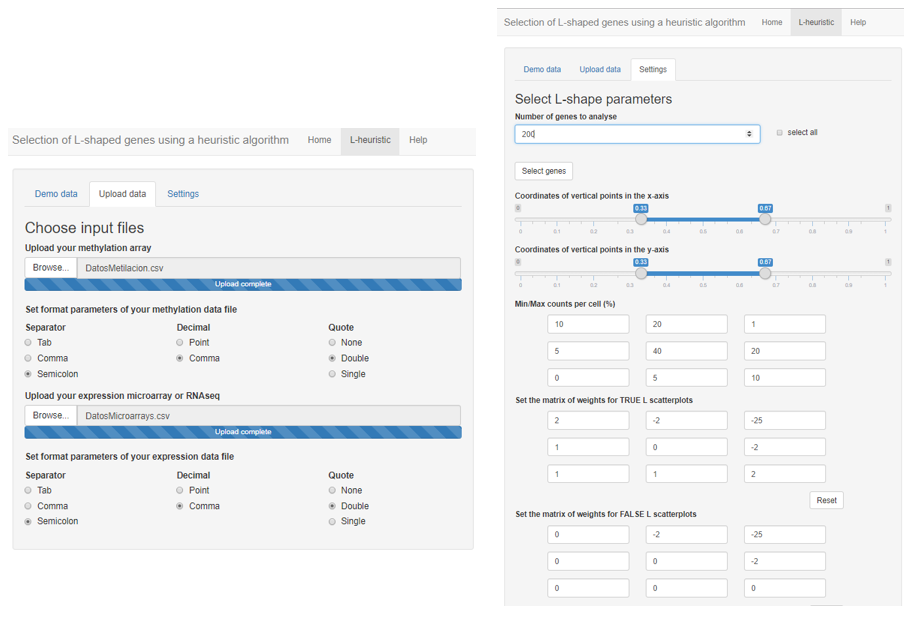
\includegraphics[height=0.8\textheight]{images/shinyApp2.png}
	\end{figure}
\end{center}

\begin{center}
	\begin{figure}[h]          
		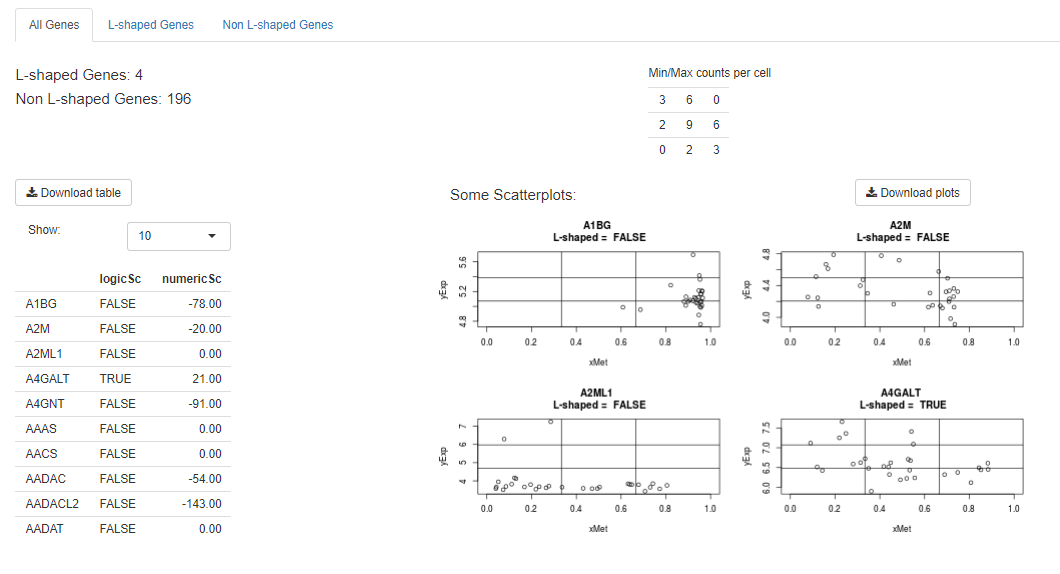
\includegraphics[width=0.9\textwidth]{images/shinyApp3.png}
	\end{figure}
\end{center}
}

\section{Discussion and conclusions}

\begin{frame}
	\frametitle{Summary of results}
 \begin{itemize}
 	\item The heuristic method is  an intuitive approach to select L-shape genes.
 	\begin{itemize}
 	\item It can be tuned easily so that different quantities of genes and L-shapes of distinct severity can be selected.
 	\item Indeed the method can be easily extended to detect other patterns such as vertical or horizontals clouds depicting distinct biological behavior. 
 	 \end{itemize} 
  
 	\item Right now the recommended approach is to apply the Naive and the Heuristic method and select the union of both sets.
 	\item A tool for using the method is available at \url{http://cinna.upc.edu:3838/alex/Lheuristic/}.
 \end{itemize} 
\end{frame}

\begin{frame}[allowframebreaks]
\frametitle{Discussion}

\begin{itemize}
	\item The standard approach is a poor one: The naive method looks for correlation (may miss L's) and relies on significance p-values for $\rho$, \textit{that only tests if this is 0 or not}: \textbf{Improving this approach through, for instance, an appropriate scoring scheme is worthwile}.
	\item We look for a statistical approach (select lists of genes ...) but most of the times researchers end up looking at a few. In this case there was only \textbf{one gene} selected for further study, which showed a clear negative correlation, but not L-shape.
	\item The method shows several weaknessess
	\begin{enumerate}
		\item The scoring system is ubiquous
		\item It is difficult to validate
		
	\end{enumerate}
\end{itemize}

\end{frame}

\begin{frame}[allowframebreaks]
	\frametitle{Some Limitations}
 \begin{itemize}
 %	\item Methylation is measured in multiple sites per gene (CpGs). Averaging the values to obtain a single methylation value per gen has been claimed to be oversimplistic.
	\item There is no TRUE/FALSE positive dataset, or at least it is very hard to consensuate one that is a list of genes related to CRC (or other diseases) and known to be regulated by methylation.
	\begin{itemize}
		\item Sensitivity and specificity cannot be computed
		\item The methods cannot be compared.
	\end{itemize}
    \item TRUE and FALSE lists can be built manually or by simulation, but \emph{How can we trust them?}
    \item Validation based on pathway analysis has come to be harder than expected because the number of GRM is often small, and belonging to distinct pathways (need very strong biological knowledge?)
\framebreak 
	\item The scoring method works conditionally on the decision that the scatterplot is declared to have an L-shape
			\begin{itemize}
			\item It is intuitive, easy to tune and easy to extend, because it allows to combine several scoring schemes.
			\item What if the decision is wrong?
			\item Doing inference based on the scores' distribution under $H_0$ is not possible (it should be if there were no binarization).
		\end{itemize}
	\item The number of parameters is high
		\begin{itemize}
			\item The method is flexible: easy to define which pattern (only L by now) and with which stringency (how restrictive) one wants to select.
			\item May be hard to optimize even if TRUE positives/negatives were available.
			\item Also hard to think of simulation scenarios.
		\end{itemize}

\item Altogether makes that, right now the methd can only be considered to be a descriptive tool.

\end{itemize} 	
\end{frame}



\begin{frame}{Acknowledgments}
	\begin{enumerate}
		\item My group ESTBIOINFO at the GME department at the University of Barcelona and the research group GRBio, led by Guadalupe Gómez.
		\item The Statistics and Bioinformatics Unit at Vall d'Hebron Institut de Recerca (VHIR).
		\item The Nanomedicine and Molecular Oncology group at VHIR, led by Dr. Diego Arango.
	\end{enumerate}
\end{frame}

\begin{frame}
	\begin{center}
		{\Huge
			Thanks for your attention!}
	\end{center}
	
	\begin{center}
		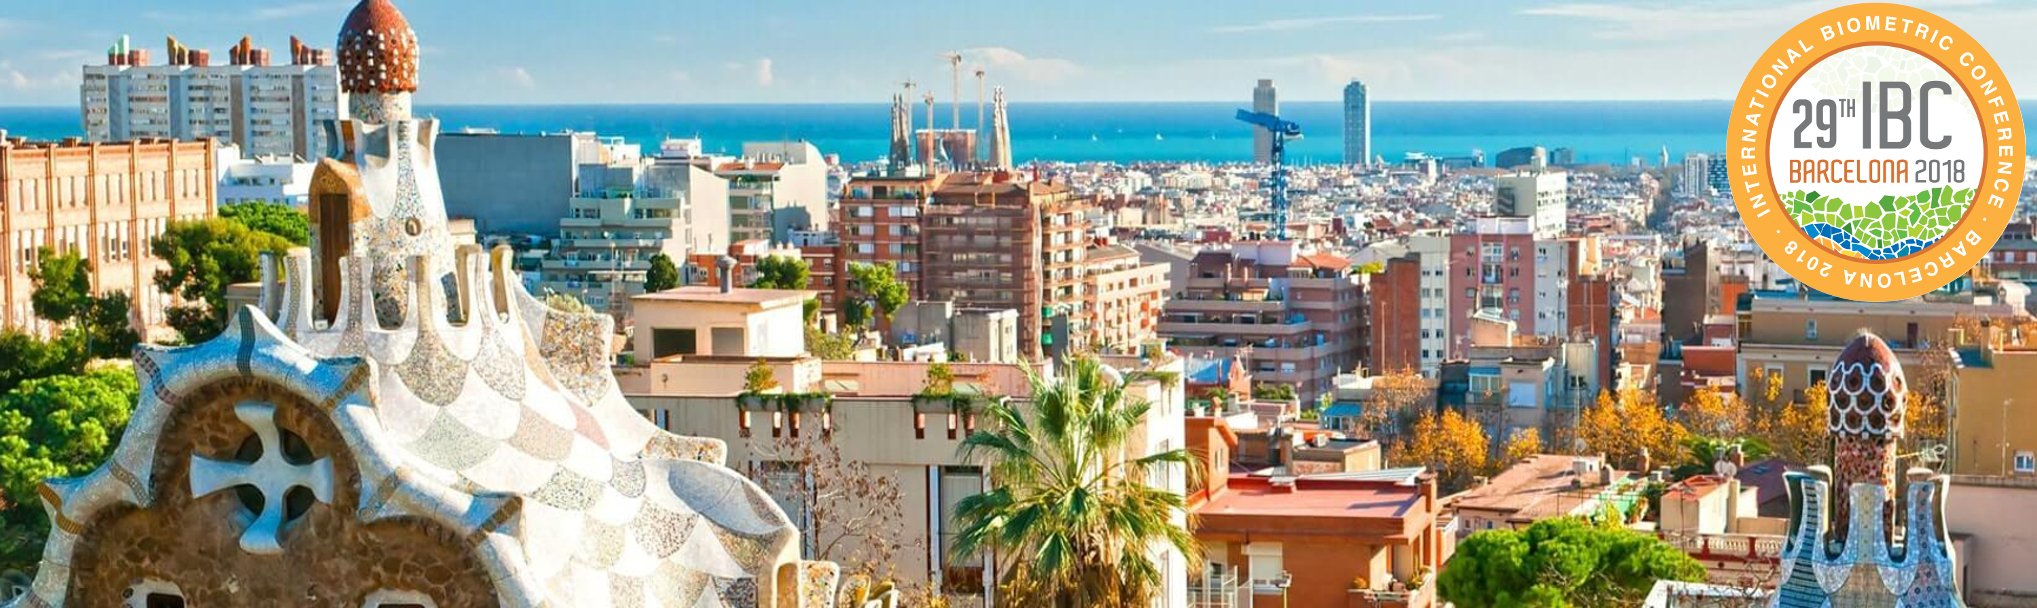
\includegraphics[width=0.9\textwidth]{./images/ibc-2018-barcelona.jpg}
	\end{center}
	
	
\end{frame}





\section*{References}
\begin{frame}\frametitle{References}
\begin{thebibliography}{9}

%\addcontentsline{toc}{chapter}{\numberline{}Bibliografía}
%
%\bibitem{cohen} J. Cohen, \emph{Statistical power analysis for the behavioral sciences} (2nd ed.). % Hillsdale,NJ: Lawrence Erlbaum, 1988.

%\bibitem{faraway} J.J. Faraway, \emph{Linear Models with R}, Chapman \& Hall/CRC, 2004.

%\bibitem{montgomery} D.C Montgomery \emph{Design and Analysis of Experiments}, John Wiley \& Sons, 2008.

%\bibitem{blog} \texttt{http://erre-que-erre-paco.blogspot.com.es/2013/04/el-codigo-body-td-font-family-sans.html}

\bibitem{Bazzocco:2015} Bazzocco, Sara. \emph{et al.} (2015) \emph{Highly Expressed Genes in Rapidly Proliferating Tumor Cells as New Targets for Colorectal Cancer Treatment}. DOI: 10.1158/1078-0432.CCR-14-2457

\bibitem{Liu:2012} Liu, Y. and Qiu, P. (2012) \emph{Integrative analysis of methylation and gene expression data in TCGA} IEEE International Workshop on Genomic Signal Processing and Statistics (GENSIPS)

\bibitem{Sanchez:2017} Sánchez-Pla, A., Ruiz de Vila, M.C:, Carmona, F., Bazzoco, S. and Arango del Corro, D. (2017). 
\emph{Integrative analysis to select genes regulated by methylation in a cancer colon study} Trends in Mathematics 2017. DOI: 10.1007/978-3-319-55639-09

\bibitem{Wilkinson:2017} Wilkinson, Leland, and Graham Wills. (2017). 
\emph{``Scagnostics Distributions''}, JCGS.

\end{thebibliography}

\end{frame}



\end{document}
